% Copyright 2007 by Mark Wibrow
%
% This file may be distributed and/or modified
%
% 1. under the LaTeX Project Public License and/or
% 2. under the GNU Free Documentation License.
%
% See the file doc/generic/pgf/licenses/LICENSE for more details.


\section{Customizing the Mathematical Engine}

\label{pgfmath-reimplement}


Perhaps you have a desire for some function that \pgfname\ does not
provide. Perhaps you are not happy with the accuracy or efficiency of
some of the algorithms that are implemented in \pgfname. In these
cases you will want to add a function to the parser or replace the
current implementations of the algorithms with your own code.

The mathematical engine was designed with such customization in mind.
It is possible to add new functions, or modify the code for
existing functions. Note, however, that whilst adding new operators
is possible, it can be a rather tricky business and is only
recommended for adventurous users.

To add a new function to the math engine the following command can be
used:

\begin{command}{\pgfmathdeclarefunction\marg{name}\marg{number of arguments}\marg{code}}

  This will set up the parser to recognize a function called
  \meta{name}. The name of the function can consist of, uppercase or
  lowercase letters, numbers or the underscore |_|. In line with
  many programming languages, a function name cannot begin with a
  number or contain any spaces.

  The \meta{number of arguments} can be any positive integer, zero,
  or the value |...|, which indicates a variable number of
  arguments. \pgfname{} treats constants, such as |pi| and |e|, as
  functions with zero arguments. Functions with more than nine
  arguments or with a variable number of arguments are a ``bit special'' and
  are discussed below.

  The effect of \meta{code} should be to set the macro
  |\pgfmathresult| to the correct value (namely to the result of the
  computation without units).  Furthermore, the function should have
  no other side effects, that is, it should not change any global
  values. As an example, consider the creation of a new function
  |double|, which takes one argument, and returns the value of that
  argument times two.

\begin{codeexample}[]
\makeatletter
\pgfmathdeclarefunction{double}{1}{
  \begingroup
    \pgf@x=#1pt\relax
    \multiply\pgf@x by2\relax
    \pgfmathreturn\pgf@x
  \endgroup
}
\makeatother
\pgfmathparse{double(44.3)}\pgfmathresult
\end{codeexample}

  The macro |\pgfmathreturn|\meta{tokens} must be
  directly followed by an |\endgroup| and will save the result of the
  computation, by defining |\pgfmathresult| as the expansion of
  \meta{tokens} (without units) outside the group, so \meta{tokens}
  must be something that can be assigned to a dimension register.

  Alternatively, the |\pgfmathsmuggle|\meta{macro} can be used. This
  must also be directly followed by an |\endgroup| and will simply
  ``smuggle'' the definition of \meta{macro} outside the \TeX-group.

	By performing computations within a \TeX-group, \pgfname{}
	registers such as |\pgf@x|, |\pgf@y| and |\c@pgf@counta|,
	|\c@pgfcountb|, and so forth, can be used at will.

  Beyond setting up the parser, this command also defines two macros
  which provide access to the function independently of the parser:

  \begin{itemize}
  \item
  |\pgfmath|\meta{function name}

  This macro will provide a ``public'' interface for the function
  \meta{function name} allowing the function to be called
  independently of the parser. All arguments passed to this macro are
  evaluated using |\pgfmathparse| and then passed on to the following
  macro:

  \item
  |\pgfmath|\meta{function name}|@|

  This macro is the ``private'' implementation of the function's
  algorithm (but note that, for speed, the parser calls this macro
  rather than the ``public'' one). Arguments passed to this macro
  are expected to be numbers without units. It is defined using
  \meta{code}, but need not be self-contained.

  \end{itemize}

  For functions that are declared with less than ten arguments,
  the public macro is defined in the same way as normal \TeX{}
  macros using, for example, |\def\pgfmathNoArgs{|\meta{code}|}|
  for a function with no arguments, or
   |\def\pgfmathThreeArgs#1#2#3{|\meta{code}|}| for a function with
   three arguments.
  The private macro is defined in the same way, and each argument
  can therefore be accessed in \meta{code}
  using |#1|, |#2| and so on.

  For functions with more than nine arguments, or functions with
  a variable number of arguments, these macros are only
  defined as taking \emph{one} argument. The public macro
  expects its arguments to be comma separated, for example,
  |\pgfmathVariableArgs{1.1,3.5,-1.5,2.6}|. Each
  argument is parsed and
  passed on to the private macro as follows:
  |\pgfmathVariableArgs@{{1.1}{3.5}{-1.5}{2.6}}|.
  This means that some ``extra work'' will be required to access
  each argument (although it is a fairly simple task).

  Note that there are two exceptions to this arrangement:
  the public versions of the |min| and |max| functions still
  take two arguments for compatibility with older versions, but
  each of these arguments can take several comma separated values.




\end{command}

  To redefine a function use the following command:

\begin{command}{\pgfmathredeclarefunction\marg{function name}\marg{algorithm code}}

  This command redefines the |\pgfmath|\meta{function name}|@| macro
  with the new \meta{algorithm code}. See the description of the
  |\pgfmathdeclarefunction| for details. You cannot change the number
  of arguments for an existing function.

\end{command}

  \pgfname{} uses the last known definition of a function within the
  prevailing scope, so it is possible for a function to be redefined
  locally. You should also remember that any |.sty| or |.tex| file
  containing any re-implementations should be loaded after |pgfmath|.

  In addition to the above commands, the following key is provided to
  quickly create simple ad hoc functions which can greatly improve
  the readability of code, and is particularly useful in \tikzname{}:

\begin{key}{/pgf/declare function=\meta{function definitions}}
  This key allows simple functions to be created locally. Its use
  is perhaps best illustrated by an example:

\begin{codeexample}[]
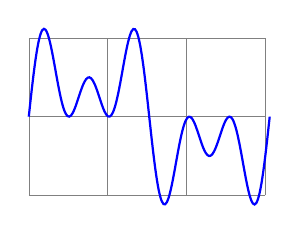
\begin{tikzpicture}
  \draw [help lines] (0,0) grid (3,2);
  \draw [blue, thick, x=0.0085cm, y=1cm,
    declare function={
      sines(\t,\a,\b)=1 + 0.5*(sin(\t)+sin(\t*\a)+sin(\t*\b));
    }]
    plot [domain=0:360, samples=144, smooth] (\x,{sines(\x,3,5)});
\end{tikzpicture}
\end{codeexample}

  Each definition in \meta{function definitions} takes the form
  \meta{name}|(|\meta{arguments}|)=|\meta{definition}|;| (note the
  semicolon at the end, this is very important). If multiple
  functions are being defined, the semicolon is used to separate
  them (\emph{not} a comma).
  The function \meta{name} can be any name that is not already a
  function name in the current scope. The list of \meta{arguments}
  are commands such as |\x|, or |\y| (it is not possible to declare
  functions that take variable numbers of arguments using this key).
  If the function takes no arguments, then the parentheses need not
  be used.
  The \meta{definition} should be an expression that can be
  parsed by the mathematical engine and should use the commands
  specified in \meta{arguments}.

  When specifying multiple functions, functions that appear later
  on in \meta{function definitions} can refer to earlier functions:

\begin{codeexample}[]
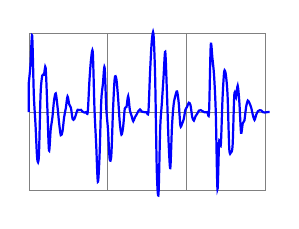
\begin{tikzpicture}[
  declare function={
    excitation(\t,\w) = sin(\t*\w);
    noise             = rnd - 0.5;
    source(\t)        = excitation(\t,20) + noise;
    filter(\t)        = 1 - abs(sin(mod(\t, 90)));
    speech(\t)        = 1 + source(\t)*filter(\t);
  }
]
  \draw [help lines] (0,0) grid (3,2);
  \draw [blue, thick, x=0.0085cm, y=1cm] (0,1) --
    plot [domain=0:360, samples=144, smooth] (\x,{speech(\x)});
\end{tikzpicture}
\end{codeexample}

\end{key}
